\chapter{Конструкторский раздел}

\section{Диаграммы состояний IDEF0}

На рисунке \ref{img:idef0} приведена диаграмма состояний IDEF0 нулевого уровня, а на рисунке \ref{img:idef1} --- диаграмма состояний IDEF0 первого уровня.

\begin{figure}[H]
	\begin{center}
		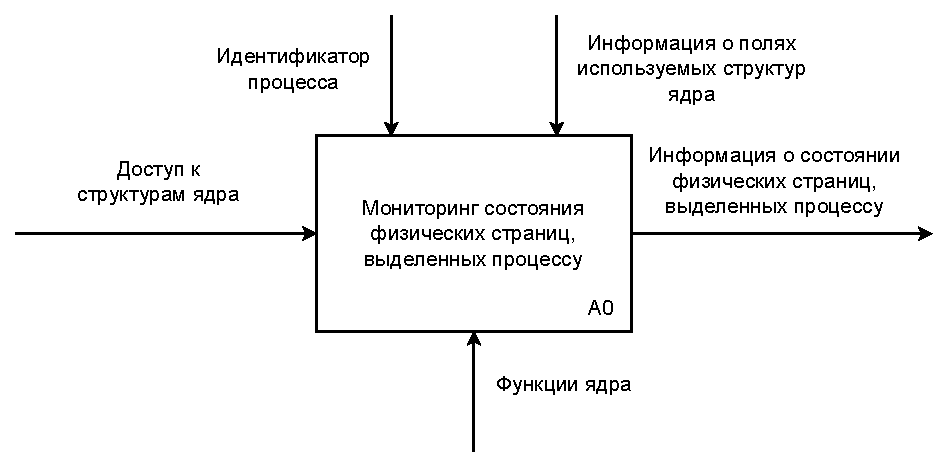
\includegraphics[scale=0.8]{inc/img/idef0.pdf}
	\end{center}
	\captionsetup{justification=centering}
	\caption{Диаграмма состояний IDEF0 нулевого уровня}
	\label{img:idef0}
\end{figure}

\begin{figure}[H]
	\begin{center}
		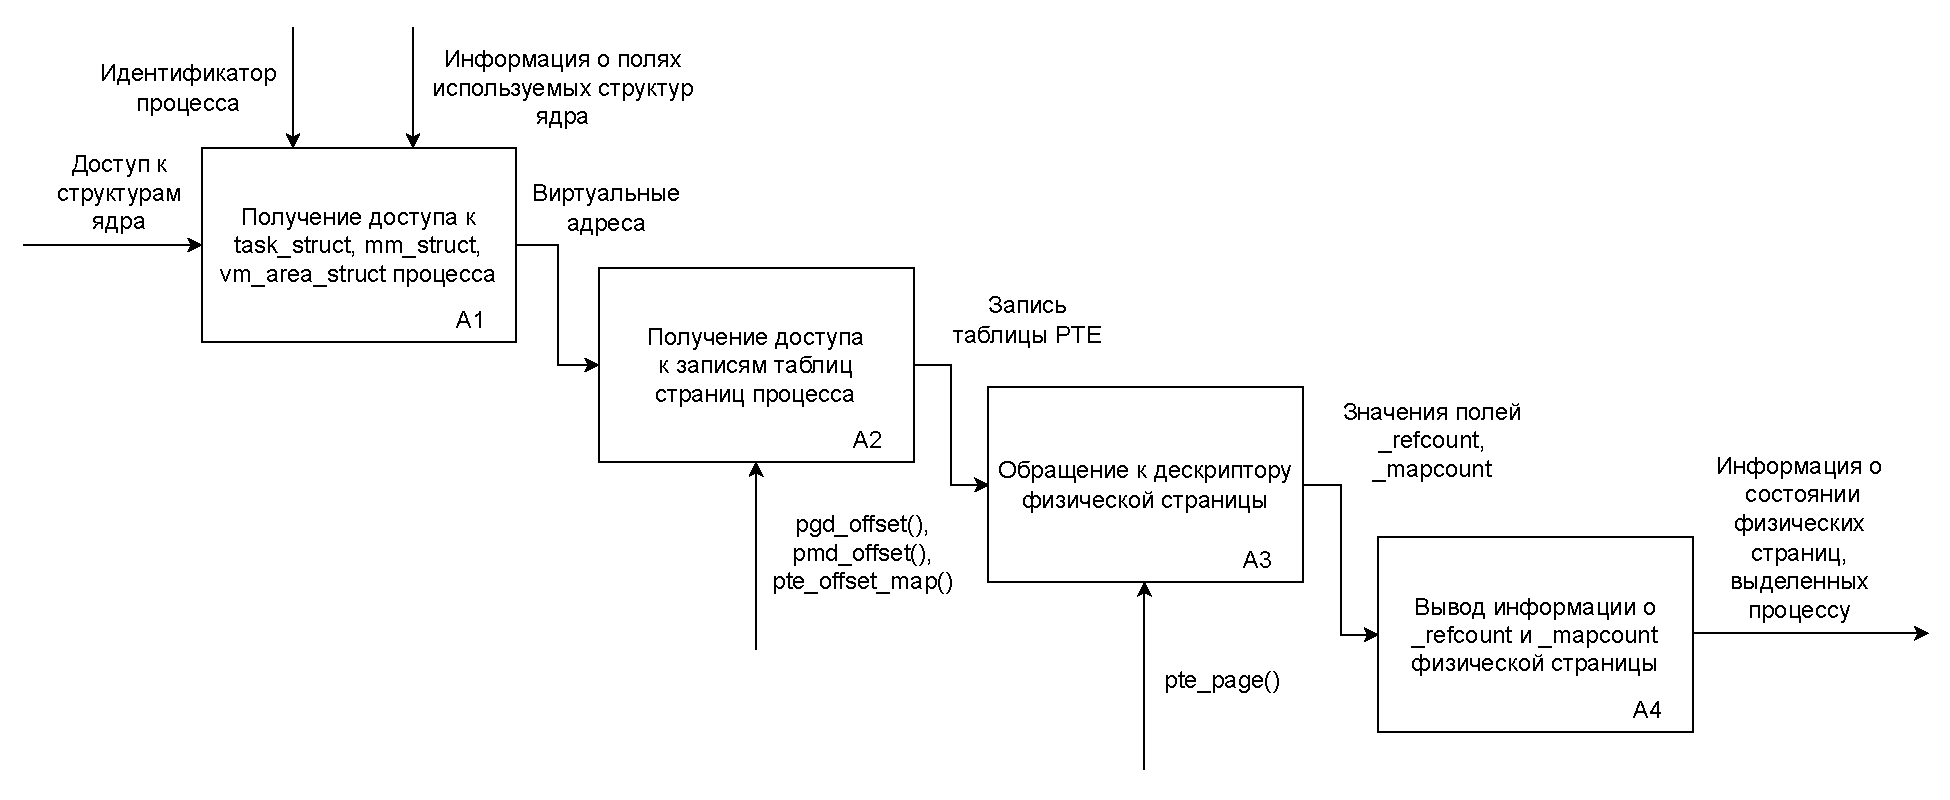
\includegraphics[scale=0.5]{inc/img/idef1.pdf}
	\end{center}
	\captionsetup{justification=centering}
	\caption{Диаграмма состояний IDEF0 первого уровня}
	\label{img:idef1}
\end{figure}

\section{Схемы алгоритмов}

\subsection{Алгоритм прохода по виртуальным адресам}

На рисунке \ref{img:trace_pages} представлена схема алгоритма прохода по виртуальным адресам.

\begin{figure}[H]
	\begin{center}
		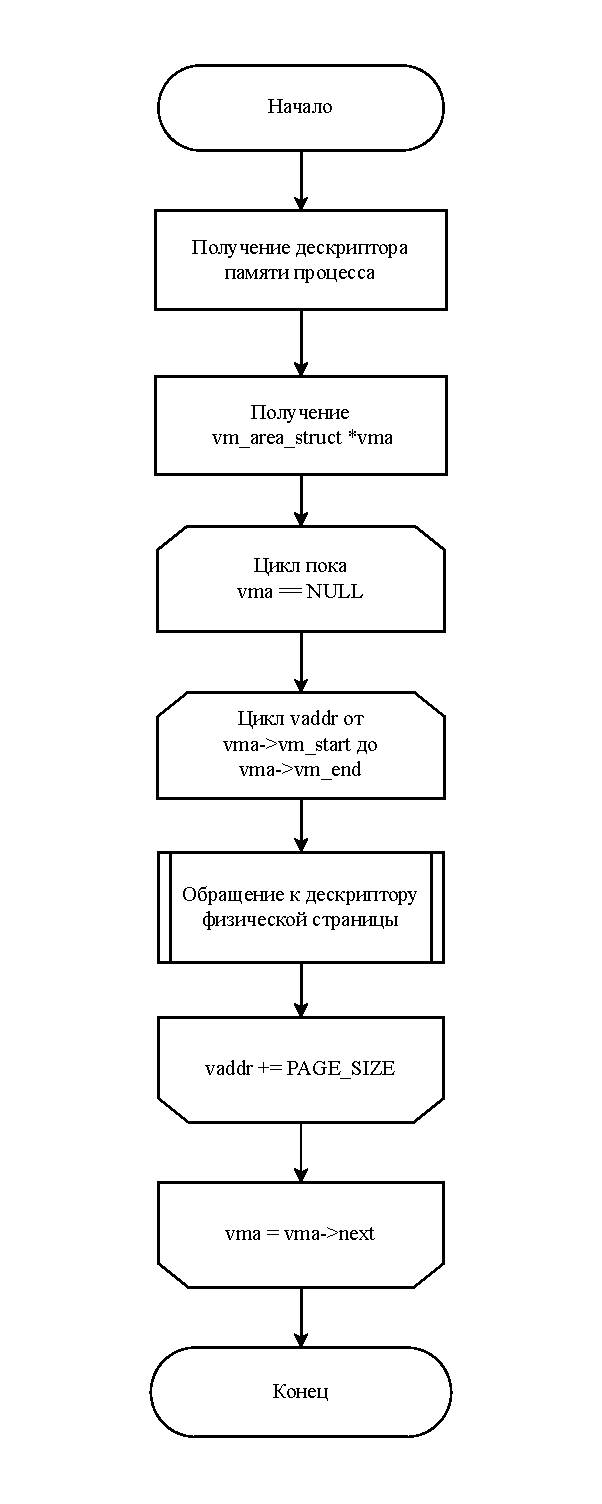
\includegraphics[scale=0.7]{inc/img/trace_pages.pdf}
	\end{center}
	\captionsetup{justification=centering}
	\caption{Проход по виртуальным адресам}
	\label{img:trace_pages}
\end{figure}

\subsection{Алгоритм получения физической страницы}

На рисунке \ref{img:get-page} показана схема алгоритма получения физической страницы.

\begin{figure}[H]
	\begin{center}
		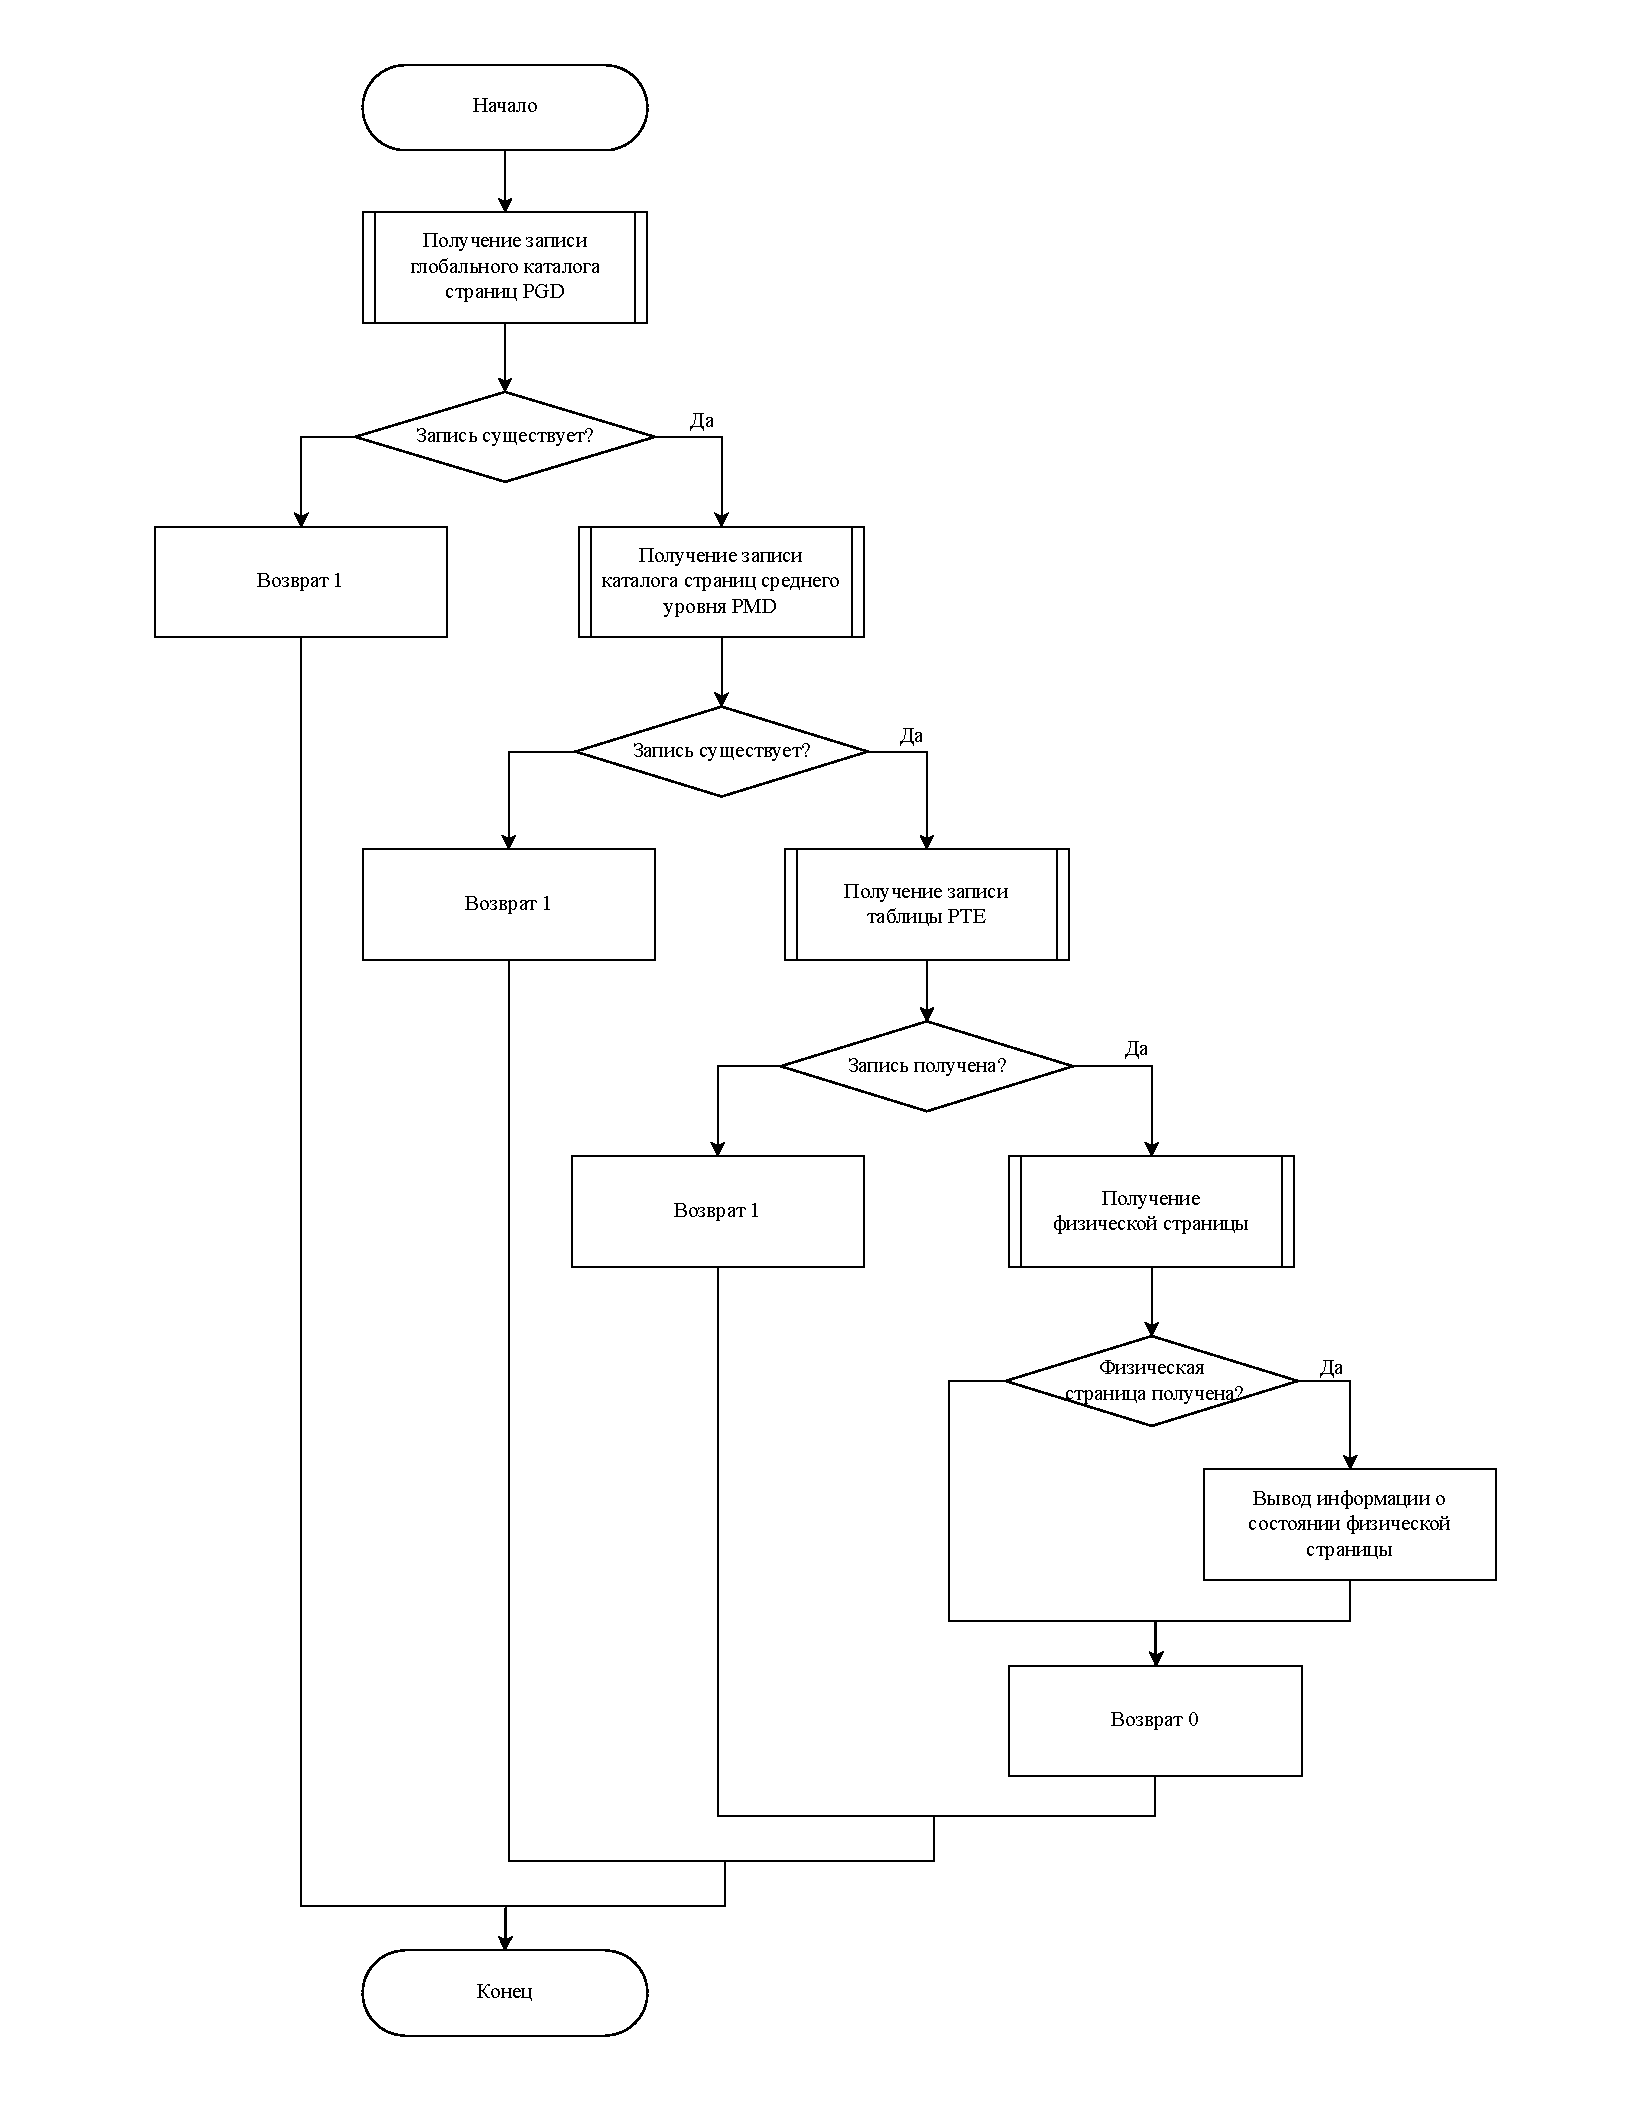
\includegraphics[scale=0.55]{inc/img/get_page.pdf}
	\end{center}
	\captionsetup{justification=centering}
	\caption{Получение физической страницы}
	\label{img:get-page}
\end{figure}

\section{Структура загружаемого модуля ядра}

На рисунке \ref{img:structure} приведена структура загружаемого модуля ядра.

\begin{figure}[H]
	\begin{center}
		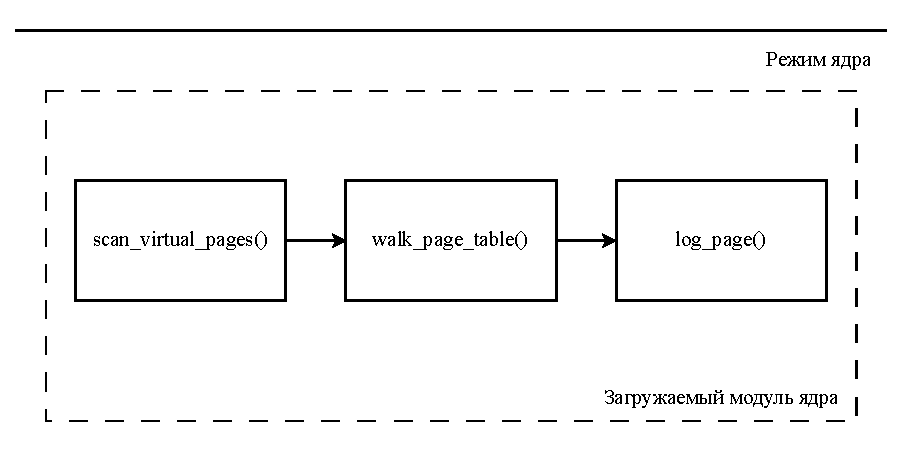
\includegraphics[scale=0.75]{inc/img/structure.pdf}
	\end{center}
	\captionsetup{justification=centering}
	\caption{Получение физической страницы}
	\label{img:structure}
\end{figure}
